\documentclass[border=10pt]{standalone}

% colour definitions
\usepackage{xcolor}
\definecolor{myblue}{rgb}{0, 0, 0.8}
\definecolor{darkgreen}{rgb}{0, 0.8, 0}

% for diagrams
\usepackage{tikz}
\usetikzlibrary{shadings, intersections, positioning, arrows}
\usetikzlibrary{decorations.pathmorphing}
\usetikzlibrary{decorations.markings}
\usetikzlibrary{decorations.pathreplacing}
\usetikzlibrary{shapes.misc}
\usetikzlibrary{shadows.blur}

\usetikzlibrary{external}
\tikzexternalize[prefix=build/]

% common things used for feynman diagrams
\tikzset{
	particle/.style={thick,draw=black, postaction={decorate},
	decoration={markings,mark=at position .5 with {\arrow[black]{triangle 45}}}}
}


\newcommand{\tauHad}{\ensuremath{\tau_\mathrm{had}}}
\newcommand{\tauhad}{\tauHad}
\newcommand{\MET}{\ensuremath{E_\mathrm{T}^\mathrm{miss.}}}

\tikzset{
	particleNoArrow/.style={thick,draw=black, postaction={decorate}}
}

\tikzset{
	Wboson/.style={decorate, draw=black,
	decoration={coil,aspect=0}}
}

\tikzset{
	gluon/.style={decorate, draw=black,
    decoration={coil,aspect=0.3,segment length=3pt,amplitude=3pt}}
 }

\begin{document}
	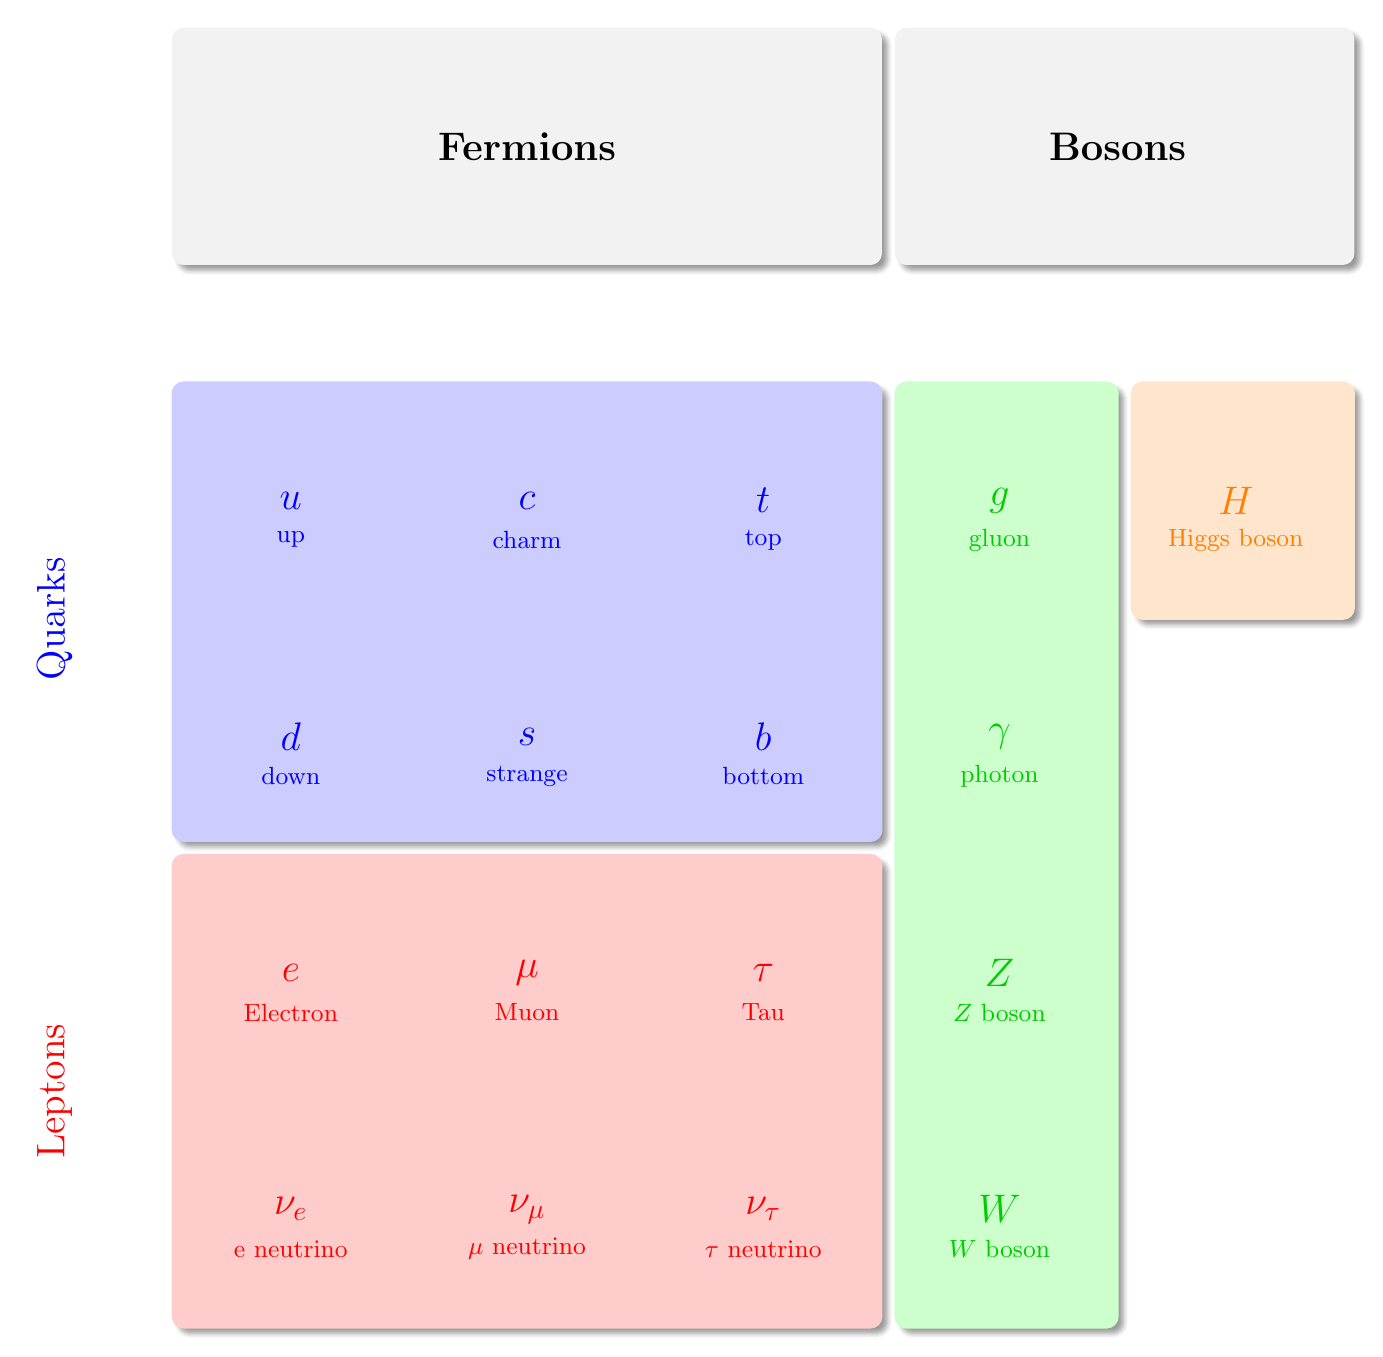
\begin{tikzpicture}[x=1.2cm, y=1.2cm]
		\newcommand{\gridstep}{2.5}
		\newcommand{\offset}{0.15}
		%\draw[thin, gray, step=\gridstep] (0, 0) grid (5 * \gridstep, 4 * \gridstep);

		%TODO: colour fills, names, shaded boxes, generations, force carrier labels

		% group particles
		\filldraw[blur shadow={shadow blur steps=5}, rounded corners, thick, color=red!20] (0 * \gridstep, 0 * \gridstep) rectangle (3 * \gridstep, 2 * \gridstep);
		\filldraw[blur shadow={shadow blur steps=5}, rounded corners, thick, color=blue!20] (0 * \gridstep, 2 * \gridstep + \offset) rectangle (3 * \gridstep, 4 * \gridstep);
		\filldraw[blur shadow={shadow blur steps=5}, rounded corners, thick, color=green!20] (3 * \gridstep + \offset, 0 * \gridstep) rectangle (4 * \gridstep, 4 * \gridstep);
		\filldraw[blur shadow={shadow blur steps=5}, rounded corners, thick, color=orange!20] (4 * \gridstep + \offset, 3 * \gridstep) rectangle (5 * \gridstep, 4 * \gridstep);

		% neutrinos
		\node at (0 * \gridstep + \gridstep / 2, 0 * \gridstep + \gridstep / 2) {\color{red}\Large$\nu_e$};
		\node at (0 * \gridstep + \gridstep / 2, 0 * \gridstep + \gridstep / 3) {\color{red}\small e neutrino};
		\node at (1 * \gridstep + \gridstep / 2, 0 * \gridstep + \gridstep / 2) {\color{red}\Large$\nu_\mu$};
		\node at (1 * \gridstep + \gridstep / 2, 0 * \gridstep + \gridstep / 3) {\color{red}\small $\mu$ neutrino};
		\node at (2 * \gridstep + \gridstep / 2, 0 * \gridstep + \gridstep / 2) {\color{red}\Large$\nu_\tau$};
		\node at (2 * \gridstep + \gridstep / 2, 0 * \gridstep + \gridstep / 3) {\color{red}\small $\tau$ neutrino};

		% leptons
		\node at (0 * \gridstep + \gridstep / 2, 1 * \gridstep + \gridstep / 2) {\color{red}\Large$e$};
		\node at (0 * \gridstep + \gridstep / 2, 1 * \gridstep + \gridstep / 3) {\color{red}\small Electron};
		\node at (1 * \gridstep + \gridstep / 2, 1 * \gridstep + \gridstep / 2) {\color{red}\Large$\mu$};
		\node at (1 * \gridstep + \gridstep / 2, 1 * \gridstep + \gridstep / 3) {\color{red}\small Muon};
		\node at (2 * \gridstep + \gridstep / 2, 1 * \gridstep + \gridstep / 2) {\color{red}\Large$\tau$};
		\node at (2 * \gridstep + \gridstep / 2, 1 * \gridstep + \gridstep / 3) {\color{red}\small Tau};

		% down type quarks
		\node at (0 * \gridstep + \gridstep / 2, 2 * \gridstep + \gridstep / 2) {\color{blue}\Large$d$};
		\node at (0 * \gridstep + \gridstep / 2, 2 * \gridstep + \gridstep / 3) {\color{blue}\small down};
		\node at (1 * \gridstep + \gridstep / 2, 2 * \gridstep + \gridstep / 2) {\color{blue}\Large$s$};
		\node at (1 * \gridstep + \gridstep / 2, 2 * \gridstep + \gridstep / 3) {\color{blue}\small strange};
		\node at (2 * \gridstep + \gridstep / 2, 2 * \gridstep + \gridstep / 2) {\color{blue}\Large$b$};
		\node at (2 * \gridstep + \gridstep / 2, 2 * \gridstep + \gridstep / 3) {\color{blue}\small bottom};
		
		% up type quarks
		\node at (0 * \gridstep + \gridstep / 2, 3 * \gridstep + \gridstep / 2) {\color{blue}\Large$u$};
		\node at (0 * \gridstep + \gridstep / 2, 3 * \gridstep + \gridstep / 3) {\color{blue}\small up};
		\node at (1 * \gridstep + \gridstep / 2, 3 * \gridstep + \gridstep / 2) {\color{blue}\Large$c$};
		\node at (1 * \gridstep + \gridstep / 2, 3 * \gridstep + \gridstep / 3) {\color{blue}\small charm};
		\node at (2 * \gridstep + \gridstep / 2, 3 * \gridstep + \gridstep / 2) {\color{blue}\Large$t$};
		\node at (2 * \gridstep + \gridstep / 2, 3 * \gridstep + \gridstep / 3) {\color{blue}\small top};

		% vector bosons
		\node at (3 * \gridstep + \gridstep / 2, 0 * \gridstep + \gridstep / 2) {\color{darkgreen}\Large$W$};
		\node at (3 * \gridstep + \gridstep / 2, 0 * \gridstep + \gridstep / 3) {\color{darkgreen}\small$W$ boson};
		\node at (3 * \gridstep + \gridstep / 2, 1 * \gridstep + \gridstep / 2) {\color{darkgreen}\Large$Z$};
		\node at (3 * \gridstep + \gridstep / 2, 1 * \gridstep + \gridstep / 3) {\color{darkgreen}\small$Z$ boson};
		\node at (3 * \gridstep + \gridstep / 2, 2 * \gridstep + \gridstep / 2) {\color{darkgreen}\Large$\gamma$};
		\node at (3 * \gridstep + \gridstep / 2, 2 * \gridstep + \gridstep / 3) {\color{darkgreen}\small photon};
		\node at (3 * \gridstep + \gridstep / 2, 3 * \gridstep + \gridstep / 2) {\color{darkgreen}\Large$g$};
		\node at (3 * \gridstep + \gridstep / 2, 3 * \gridstep + \gridstep / 3) {\color{darkgreen}\small gluon};

		% scalar boson (Higgs)
		\node at (4 * \gridstep + \gridstep / 2, 3 * \gridstep + \gridstep / 2) {\color{orange}\Large$H$};
		\node at (4 * \gridstep + \gridstep / 2, 3 * \gridstep + \gridstep / 3) {\color{orange}\small Higgs boson};

		% fermion generations
		\filldraw[blur shadow={shadow blur steps=5}, rounded corners, color=gray!10] (0 * \gridstep, 4 * \gridstep + \gridstep / 2) rectangle (3 * \gridstep, 5 * \gridstep + \gridstep / 2);
		\node at (1 * \gridstep + \gridstep / 2, 5 * \gridstep) {\Large\textbf{Fermions}};

		%\node at (0 * \gridstep + \gridstep / 2, 4 * \gridstep + \gridstep / 2) {1};
		%\node at (1 * \gridstep + \gridstep / 2, 4 * \gridstep + \gridstep / 2) {2};
		%\node at (2 * \gridstep + \gridstep / 2, 4 * \gridstep + \gridstep / 2) {3};

		% bosons
		\filldraw[blur shadow={shadow blur steps=5}, rounded corners, color=gray!10] (3 * \gridstep + \offset, 4 * \gridstep + \gridstep / 2) rectangle (5 * \gridstep, 5 * \gridstep + \gridstep / 2);
		\node at (3 * \gridstep + \gridstep, 5 * \gridstep) {{\Large\textbf{Bosons}}};

		% leptons
		\node[rotate=90] at (-1 * \gridstep / 2, 1 * \gridstep) {\color{red}\Large{Leptons}};

		% quarks
		\node[rotate=90] at (-1 * \gridstep / 2, 3 * \gridstep) {\color{blue}\Large{Quarks}};

	\end{tikzpicture}
\end{document}
